
\documentclass[12pt,3p]{report}
\usepackage[left=2cm, right=2cm, top=4cm]{geometry} 

\makeatletter
\def\ps@pprintTitle{%
 \let\@oddhead\@empty
 \let\@evenhead\@empty
 \def\@oddfoot{\centerline{\thepage}}%
 \let\@evenfoot\@oddfoot}
\makeatother

\newcommand{\tabitem}{~~\llap{\textbullet}~~}

\usepackage{multicol,lipsum}
\usepackage{amssymb}
\usepackage{makecell}
\usepackage{graphicx}
\usepackage{amsmath}
\usepackage{fancyhdr}
\graphicspath{ {./} }


\begin{document}


\pagestyle{fancy}
\lhead{}
\rhead{Group 15, MCEN30019 Assignment 2}

\title{
	\huge Component Selection and Evaluation\\
	\small Prosthetic Hand Development for Landmine Victims \\
	\vspace{0.5cm}
	\vspace{1cm}
	\large Group 15
}

\author{
	George Juliff\\
	\texttt{624946}
	\and
	Thomas Miles\\
	\texttt{626263}
	\and
	Adam Kues\\
	\texttt{833407}
	\and
	Lucas Brouwer\\
	\texttt{1005958}
}


\pagenumbering{gobble}
\maketitle
\vspace{2cm}

\begin{abstract}
This report describes the methodology used during the pre-prototyping phase for the mechanical design of a low cost robotic prosthetic hand. Several feasible subsystem designs are proposed and their suitability in combination is determined using a set of objective evaluation functions. Due to the systematic nature of this early design process, the system's initial concept design is shown to be well optimised to best achieve our design targets while accounting for limitations in cost and manufacturing capability specific to the product.
\end{abstract}

\pagebreak

\tableofcontents

\pagebreak

\pagenumbering{arabic}

\part{Forward}
\section{Summary of Design Criteria}
	\subsection{Essential}	\label{ess}
	
		\begin{center}
	\begin{tabular}{ |c|c|c| } 
 \hline
 Criterion & Objectives & Evaluation Function \\ 
 \hline\hline
 $E_1$ & $Obj3$ & \makecell[l]{Met if: \\
 \tabitem Portion attached to forearm weighs less than 500g. \\
 \tabitem Unit does not cause pain, irritation or significant discomfort. \\
 \tabitem Forearm size does not exceed 1.1 times natural forearm width.} \\
 \hline
 $E_2$ & $Obj_2$ & \makecell[l]{Met if: \\
 \tabitem Unit costs less than \$500AU to manufacture. \\
 \tabitem Unit takes less than 2 weeks to manufacture.} \\ 
 \hline
 $E_3$ & $Obj_{1,3}$ & \makecell[l]{Met if: \\
 %\tabitem Unit palmer pinch force is greater than 65N. \\
 \tabitem Unit closes at 115$^{\circ}$/s. \\
 \tabitem Unit has a idle battery life of 10 hours. \\
 \tabitem Software has gesture classification accuracy above 90\%.} \\
 \hline
 $E_4$ & $Obj_{2,3}$ & \makecell[l]{Met if: \\
 \tabitem Unit IP 54 rated on exposed sections. \\
 \tabitem Unit components have an expected 1 year lifespan.} \\ 
 \hline
		\end{tabular}
	\end{center}

	\subsection{Desirable} \label{des}
		\begin{center}
			\begin{tabular}{ |c|c|c|c| } 
 \hline
 Criterion & Objectives & Evaluation Function & Definitions \\ 
 \hline\hline
 $D_1$ & $Obj_1$ & $\text{min} \left \{\dfrac{M_{RF}}{M_{RF_{max}}},1 \right \}$ &  \makecell[l]{
  \vspace{1mm}
 $M_{RF}$: Impact strength (N impulsive) \\
 $M_{RF_{max}}$: 140N
 \vspace{1mm}
 } \\
 \hline
 
 $D_2$ & $Obj_3$ & $\text{max} \left \{1-\dfrac{M_L}{M_{L_{max}}}, 0 \right \}$ &  \makecell[l]{
 \vspace{2mm}
 $M_L$: Noise in actuation (dB) \\
 $M_{L_{max}}$: 50dB
 } \\
 \hline

 $D_3$ & $Obj_1$ & $D_3 =  \cfrac{\sum_{n=1}^{n=\text{DOF}} \left(k_n \cdot \text{min}\{\frac{M_{RS}}{M_{RS_{max}}},1\} \right)}{\text{DOF}}$ &  \makecell[l]{
 $M_{RS_n}$: Rotation speed (degree n, $^\circ$/s). \\
 $M_{RS_{max}}$: $230^\circ$/s
 } \\
 \hline
 $D_4$ & $Obj_3$ & $D_4 = \cfrac{p_{range}}{100} \times d  \times I $ &  \makecell[l]{
 **variable definitions***
 } \\
 
 \hline
		\end{tabular}
	\end{center}



\pagebreak

\part{Mechanical Design}
\begin{multicols}{2}

	\section{Fingers}
TODO explain general material selection reasoning (in that they are all printed n' shit)
	
	
		\subsection{Transmission}
		
		
			\begin{enumerate}
			\item \textbf{Flexor tendon through sheaths} {

%TODO figures are fukd
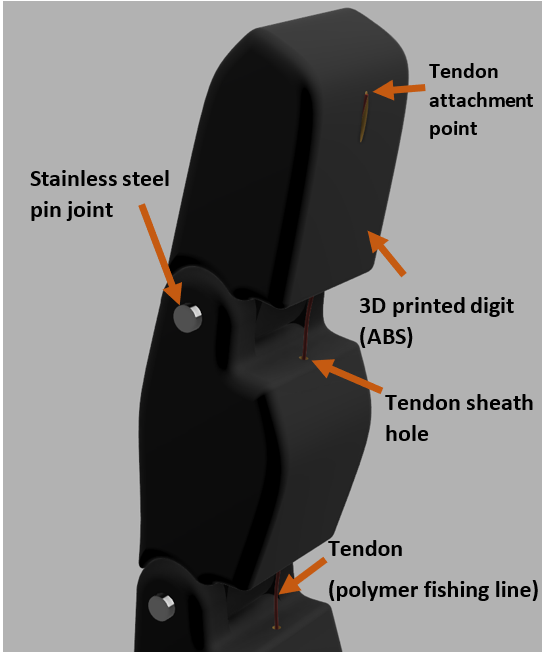
\includegraphics[scale=0.5]{tendon.PNG}
			
				This method of articulating the finger relies on closely mimicking a real finger and using a tendon to provide one degree of freedom to each finger and the thumb. These tendons will be controlled by motors either in the hand or wrist. Multiple fingers can be attached to a single motor, reducing degrees of freedom, but potentially improving other characteristics such as weight.
				
			}
			\item \textbf{Felxor tendon using pulleys} {
							
				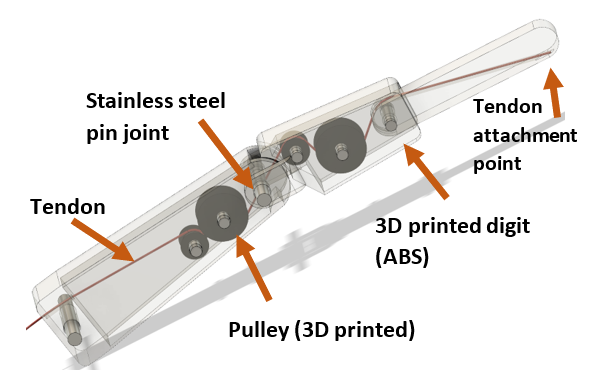
\includegraphics[scale=0.5]{pulley.PNG}
				A more novel tendon design based on xxCITATIONxx, which provides a slight mechanical advantage over design 1, and has a smoother closing action since pulley placement distributes load between finger digits more evenly. 
			}
			\item \textbf{Geared metacarpo-phalangeal joint} {
			
				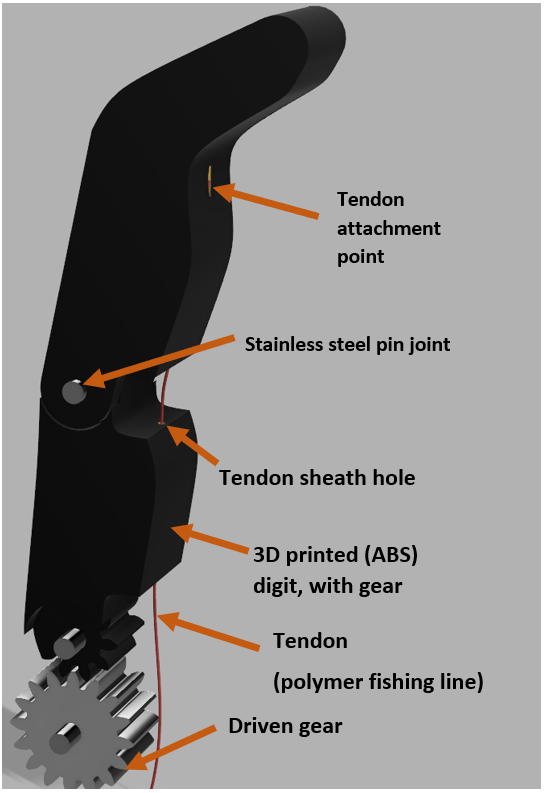
\includegraphics[scale=0.5]{gear.PNG}
				This method of articulating the finger ensures the finger closes evenly, using a tendon for the upper joint, attached to the same motor that drives the gear that closes the lower joint, prevents one joint closing at a different rate to the others. Furthermore, transmission of power to the finger via a gear will allow for actuation in both directions, and is less prone to failure than fishing line, which may snap under extreme loads.
			}		
			\end{enumerate}
			
		\subsection{Joints}
		
		\begin{enumerate}
		\item \textbf{Pin joint} {
		
		As pictured above TODO
		}
		\item \textbf{Elastic joint} {
		
		xxCITATIONxx type
		}
		\item \textbf{Silicone} {
		
		fully rubber TODO
		}
		\end{enumerate}

	


\subsection{Degrees of freedom and constraints}
		
		In order to satisfy essential criteria $E_3$, the hand must be able to, at minimum, open and close with a force of 65 newtons. This can be achieved using a single degree of freedom (DOF), closing all fingers simultaneously. Each finger transmission design explored have a single degree of freedom for this reason. 
		
		The total number of constraints and DOF's for a finger depends on the joint morphology.



	\section{Thumb}
	
		\subsection{Degrees of freedom and constraints}

		
		\subsection{Transmission of opposable joint}
			\begin{enumerate}
			\item \textbf{Rigid} {
			
			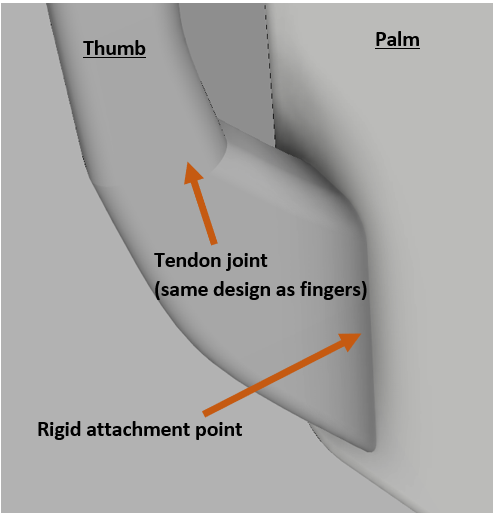
\includegraphics[scale=0.55]{rigid_thumb.PNG}
						This design allows for the lower thumb joint and the palm to be 3D printed as part of the same piece, reducing assembly difficulty.
			}

			\item \textbf{Manual operation} {
				
				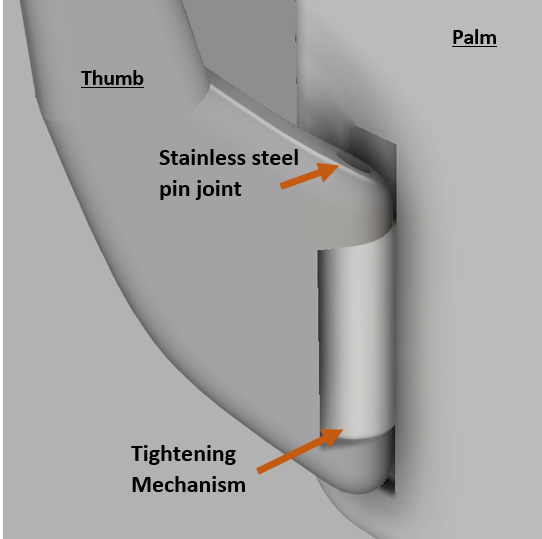
\includegraphics[scale=0.45]{man_thumb.PNG}
				This joint is manually articulated using the operator's other hand, allowing different thumb orientations to tackle a wider range of tasks. For this to be useful however, the joint needs to be stiff enough to remain in a set position during use. This can be achieved either using a very snug fit on the pin joint, have a thread on the pin joint by which the user can tighten a nut to lock it in place, or using a spring-ratchet system similar to that in figure: TODO
			}
			\item \textbf{Geared} {
				
				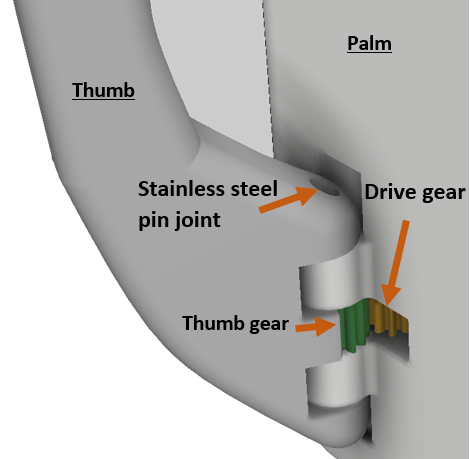
\includegraphics[scale=0.5]{Driven_thumb.PNG}
				This method is analogous to the geared joint finger design, however it allows one more degree of freedom since the second joint can be operated independently of opposable rotation. 
			}		
			\end{enumerate}	
		
		
		
	\section{Wrist}
	
		\subsection{Degrees of freedom and constraints}
		TODO briefly explain (with cite) why this is needed and why only 1 DOF is reasonable
		
		\subsection{Transmission}	
		
			
			\begin{enumerate}
			\item \textbf{Rigid} {
			
				A fixed wrist joint is the simplest to manufacture, and will reduce the overall weight due to the need for one fewer motors.
			}	
			\item \textbf{Planetary gearbox} {

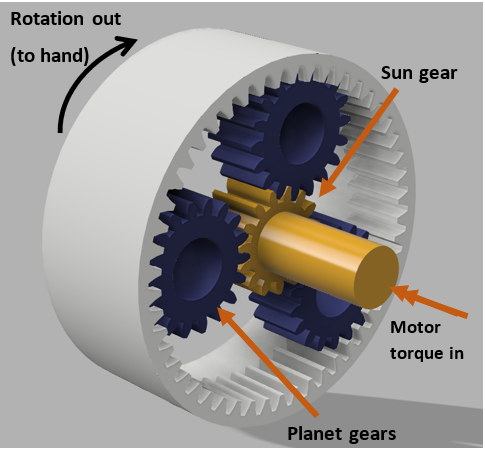
\includegraphics[scale=0.6]{planet.PNG}
The planetary gearbox design does not require a bearing since the outer ring can be embedded into the hand side of the prosthetic, while planet gears can be made captive using a herringbone tooth pattern. It also allows for a very high gear ratio without the need for multiple step-downs, since 3D printing gives us the ability to manufacture any sized gears required. Due to the number of gears, inaccuracy in 3D printed teeth, and rate of rotation of the sun gear, a planetary system will be a fair amount louder than alternate methods during operation.
			}	
			\item \textbf{Belt Drive} {

Belt drives can mitigate the noise factor associated with printed plastic on plastic gears, however achieving high gear ratios may require more than one belt for the same ratio a planetary gearbox could achieve. Furthermore, physical space within the arm may be a concern, since the rotation required is in the axis of the arm, the belt and pulley are limited in size.
			}	
			\end{enumerate}


	
	
	\section{Socket}
		
		\subsection{Solid, generic}
		

		
		\subsection{Solid, 3D printed}
		
		
		
		\subsection{Non-rigid/Strap on}
		
				\pagebreak
			\end{multicols}	
	\section{Evaluation}
\begin{tabular}{|c|c|c|c|c|c|c|c|c||c|}
\hline 
 & $E_1$ & $E_2$ & $E_3$ & $E_4$ & $D_1$ & $D_2$ & $D_3$ & $D_4$ & $D_{overall}$ \\ 
\hline 
Finger 1. & • & • & • & • & • & • & • & • & •\\ 
\hline 
Finger 2. & • & • & • & • & • & • & • & • & •\\ 
\hline 
Finger 3. & • & • & • & • & • & • & • & • & •\\ 
\hline 
Joint 1. & • & • & • & • & • & • & • & • & •\\ 
\hline 
Joint 2. & • & • & • & • & • & • & • & • & •\\ 
\hline 
Joint 3. & • & • & • & • & • & • & • & • & •\\ 
\hline 
Thumb 1. & • & • & • & • & • & • & • & • & •\\ 
\hline 
Thumb 2. & • & • & • & • & • & • & • & • & •\\ 
\hline 
Thumb 3. & • & • & • & • & • & • & • & • & •\\ 
\hline 
Wrist 1. & • & • & • & • & • & • & • & • & •\\ 
\hline 
Wrist 2. & • & • & • & • & • & • & • & • & •\\ 
\hline 
Wrist 3. & • & • & • & • & • & • & • & • & •\\ 
\hline 
Socket 1. & • & • & • & • & • & • & • & • & •\\ 
\hline 
Socket 2. & • & • & • & • & • & • & • & • & •\\ 
\hline 
Socket 3 & • & • & • & • & • & • & • & • & •\\
\hline
\hline 
 & $E_1$ & $E_2$ & $E_3$ & $E_4$ & $D_1$ & $D_2$ & $D_3$ & $D_4$ & $D_{overall}$ \\
\hline 
Full 1 & • & • & • & • & • & • & • & • & • \\ 
\hline 
Full 2 & • & • & • & • & • & • & • & • & • \\ 
\hline 
Full 3 & • & • & • & • & • & • & • & • & • \\ 
\hline 
\end{tabular} 




\pagebreak
\part{Actuator Selection}

\begin{multicols}{2}

	\section{Preamble}

		In the proposed design we evaluate the motors against we aim for 4 degrees of freedom; 1 for the fingers,
		two for the thumb, and one for the wrist. However, the wrist is manually controlled, leaving 3 motors.
		 This gives the most power to the prosthetic user and allows
		them to perform almost any grip achievable by a human hand. The cost of this
		flexibility is that we will require three motors in the prosthesis, which has
		cost and space availability impacts.

	\section{Motors}
	
		\subsection{SG90 Servo Motor}
	
		A micro motor commonly used with Arduino, the motor is small, lightweight
		and widely available and is precisely controllable. Because it is a servo
		motor, it contains an inbuilt potentiometer which allows each actuated finger
		to know its precise location in space at any time, and provides a easy digital
		interface over PWM for control.

		\begin{itemize}
		    \item[\checkmark] $E_1$ is met. The weight of the individual motors are 14.7g each, meaning that 3 motors would consume a reasonable 44.1g of the entire mass budget. Other conditions in $E_1$ are independent of motor choice.
		    \item[\checkmark] $E_2$ is met. The price of the SG90 hovers around \$11.18 AUD, making it a cheap and viable option for use in the prosthesis. The manufacturing time is not affected by the choice of motor, so this criterion is met too.
		    \item[\checkmark] $E_3$ is met. The nominal speed of 0.1s/60$^{\circ}$ corresponds to 600$^{\circ}/s$. This is more than enough for closing, which is likely to meet very little resistive torque. The unit draws 5V, which is providable over 10 hours by, for example, \cite{coreelectronics} which provides 5V for 100mAh which corresponds to 100mA for 10 hours. 
		    \item[\checkmark] $E_4$ is provisionally met. The manufacturer does not provide any expected lifespan specifications.
		    \item $D_1$ is irrelevant to the motor selection, as the motor is not withstanding large impact.
		    \item $D_2$ is relevant, but the manufacturer provides no information on the sound of the design.
			\item $D_3$ is relevant. For simplicity, we calculate 1 DOF and assume $k_n = 1$. Assuming the motor faces minimal resistance from the prosthetic shell the motor operates at a nominal speed of 0.1s/60$^{\circ}$ or 600$^{\circ}/s$. Taking $R_{finger} = 110$mm and $R_{motor} = 25$mm and assuming linear motion equality we have the rotation speed of the finger as $600\cdot\frac{25}{110} \approx 136^\circ$/s which is less than $M_{RS_{max}}= 230^\circ$/s. Thus $D_3 = \frac{136}{230} = 0.59$.
		    \item $D_4$ is about the aesthetic in the design, and measures the deviations of the design from the dimensions of a
		    human hand. Since the motors are concealed inside the palm, and the dimensions of the motor 12x23x32mm are small enough to be concealed, this criterion is independent of motor choice.

		\end{itemize}
	
		\subsection{EC-max 22 mm, brushless, 25W}
		
		The small design of the flat DC motors makes the Maxon motor a very interesting option. Although it's really compact the maxon flat DC motor has a max radial load of 16 Newtons. The motor is small compared to different motors and has a weight of just 83 grams which makes it very easy to implement into our design. The Maxon motors look very promising but only have one big issue: the price. One Maxon motor will cost as much as 5 or more regular stepper motors. 

		\begin{itemize}
		    \item[$\times$] $E_1$ is not met. The weight of the individual motors are 110g each, meaning that 3 motors would alone come close to exceeding our 500g limit. Even two motors for two degrees of freedom would erode a significant amount of our weight budget. One solution could be to mount the motors on the forearm where the weight does not have as much impact, but this would make cable-based actuation very difficult as the model would have to run cables along the length of the forearm.
		    \item[$\times$] $E_2$ is not met. The price of any Maxon motors is too high (\$306.51) to meet this criterion. Replacing any motor will also be very expensive but the lifespan of a single motor will be high. Repairing the motors can be very difficult and will take more time than replacing them.
		    \item[$\times$] $E_3$ is not met. The nominal speed of 9800 rpm is more than enough to ensure a closing spped of 115$^{\circ}$/s. However, we cannot guarantee a battery life of 10 hours. Using a top end LiPo battery that runs at 3.7V 6000mAh, this would mean we need to only draw 600mA to last ten hours; but this is not sufficient for the motor which runs at 25W.
		    \item[\checkmark] $E_4$ is met. Maxon motors are a top end motor brand and have a lifespan lasting longer than a year.  If the motors are treated and serviced right the lifespan can be made even longer. Waterproofing is irrelavent for motor choice, so we do not consider that criteria.
		    \item $D_1$ is irrelevant to the motor selection, as the motor is not withstanding large impact.
		    \item $D_2$ is relevant, but the manufacturer provides no information on the sound of the deisgn.
		    \item $D_3$ is relevant. For simplicity, we calculate 1 DOF and assume $k_n = 1$. Assuming the motor faces minimal resistance from the prosthetic shell the motor operates at a nominal speed of 9800 rpm, which $\gg M_{RS_{max}}= 230^\circ$/s. Thus $D_3 = 1.0$.
		    \item $D_4$ is about the aesthetic in the design, and measures the deviations of the design from the dimensions of a
		    human hand. Since the motors are concealed inside the palm, and the dimensions of the motor 22x22x48mm are small enough to be concealed, this criterion is independent of motor choice.

		\end{itemize}
		
		\subsection{SY20STH30-0604A Stepper Motor}

		This stepper motor has a high torque and is very responsive to new inputs. Being a stepper motor, it affords fine control
		over the rotation angles which suits precise finger gripping movements for the prosthesis.

		\begin{itemize}
		    \item[\checkmark] $E_1$ is met. The weight of a single motor is given as 60g, meaning that 3 motors consumes a non-negligible but acceptable 180g of our mass budget. The other criteria are met trivially because the motor choice has no bearing on them.
		    \item[\checkmark] $E_2$ is met. They cost about \$21 AUD each, which is an acceptable cost and leaves enough money for other parts of the prosthesis. The manufacturing time is not affected by the choice of motor, so this criterion is met too.
		    \item[\checkmark] $E_3$ is met. Although the RPM is not given specifically (since stepper motors are not known for their speed), we can use \cite{stepcalc} to calculate it, which gives us $3441.6^\circ$/s. Assuming the linear motion of the rotor and finger are equal and taking $R_{finger} = 110$mm and $R_{motor} = 16$mm, we have rotation of $3441.6\cdot\frac{16}{110} \approx 500^\circ$/s which is more than enough. The unit draws 4V, which is providable over 10 hours by \cite{coreelectronics} which provides 5V for 100mAh which corresponds to 100mA for 10 hours. 
		    \item[\checkmark] $E_4$ is provisionally met. The manufacturer does not provide any expected lifespan specifications.
		    \item $D_1$ is irrelevant to the motor selection, as the motor is not withstanding large impact.
		    \item $D_2$ is relevant, but the manufacturer provides no information on the sound of the design.
		    \item $D_3$ is relevant. For simplicity, we calculate 1 DOF and assume $k_n = 1$. As attained before, the unloaded motor can operate a finger at $500 > 230^\circ$/s. Thus $D_3 = 1.0$.
		    \item $D_4$ is about the aesthetic in the design, and measures the deviations of the design from the dimensions of a
		    human hand. Since the motors are concealed inside the palm, and the dimensions of the motor 20x20x30mm are small enough to be concealed, this criterion is independent of motor choice.
		 \end{itemize}

\end{multicols}

	\newpage
	\section{Evaluation}

	\begin{tabular}{|c|c|c|c|c|c|c|c|c||c|}
		\hline 
		& $E_1$ & $E_2$ & $E_3$ & $E_4$ & $D_1$ & $D_2$ & $D_3$ & $D_4$ & $D_{overall}$ \\ 
		\hline 
		SG90            & 1.00 & 1.00 & 1.00 & -- & -- & -- & 0.59 & -- & 0.59 \\
		EC-max          & 0.00 & 0.00 & 0.00 & -- & -- & -- & 1.00 & -- & 1.00 \\
		SY20STH30-0604A & 1.00 & 1.00 & 1.00 & -- & -- & -- & 1.00 & -- & 1.00 \\
		\hline
	\end{tabular} 


	In the evaluation of $D_{overall}$, we rescale back to a 0 to 1 range to compensate for some fields not being included as they are not applicable. We can clearly see that the SY20STH30-0604A is best for our design as it satisfies all essential criteria and scores the best in the relevant desirable criteria.


\newpage
\appendix

\bibliography{proj}{}
\bibliographystyle{plain}


\end{document}
